\section*{Research Update}
Thank you for the opportunity to provide a brief update on our progress since the submission of the MIRA proposal earlier this year.  
\begin{floatingfigure}[lt]{3.5in}
\vspace{-8mm}
\begin{center}
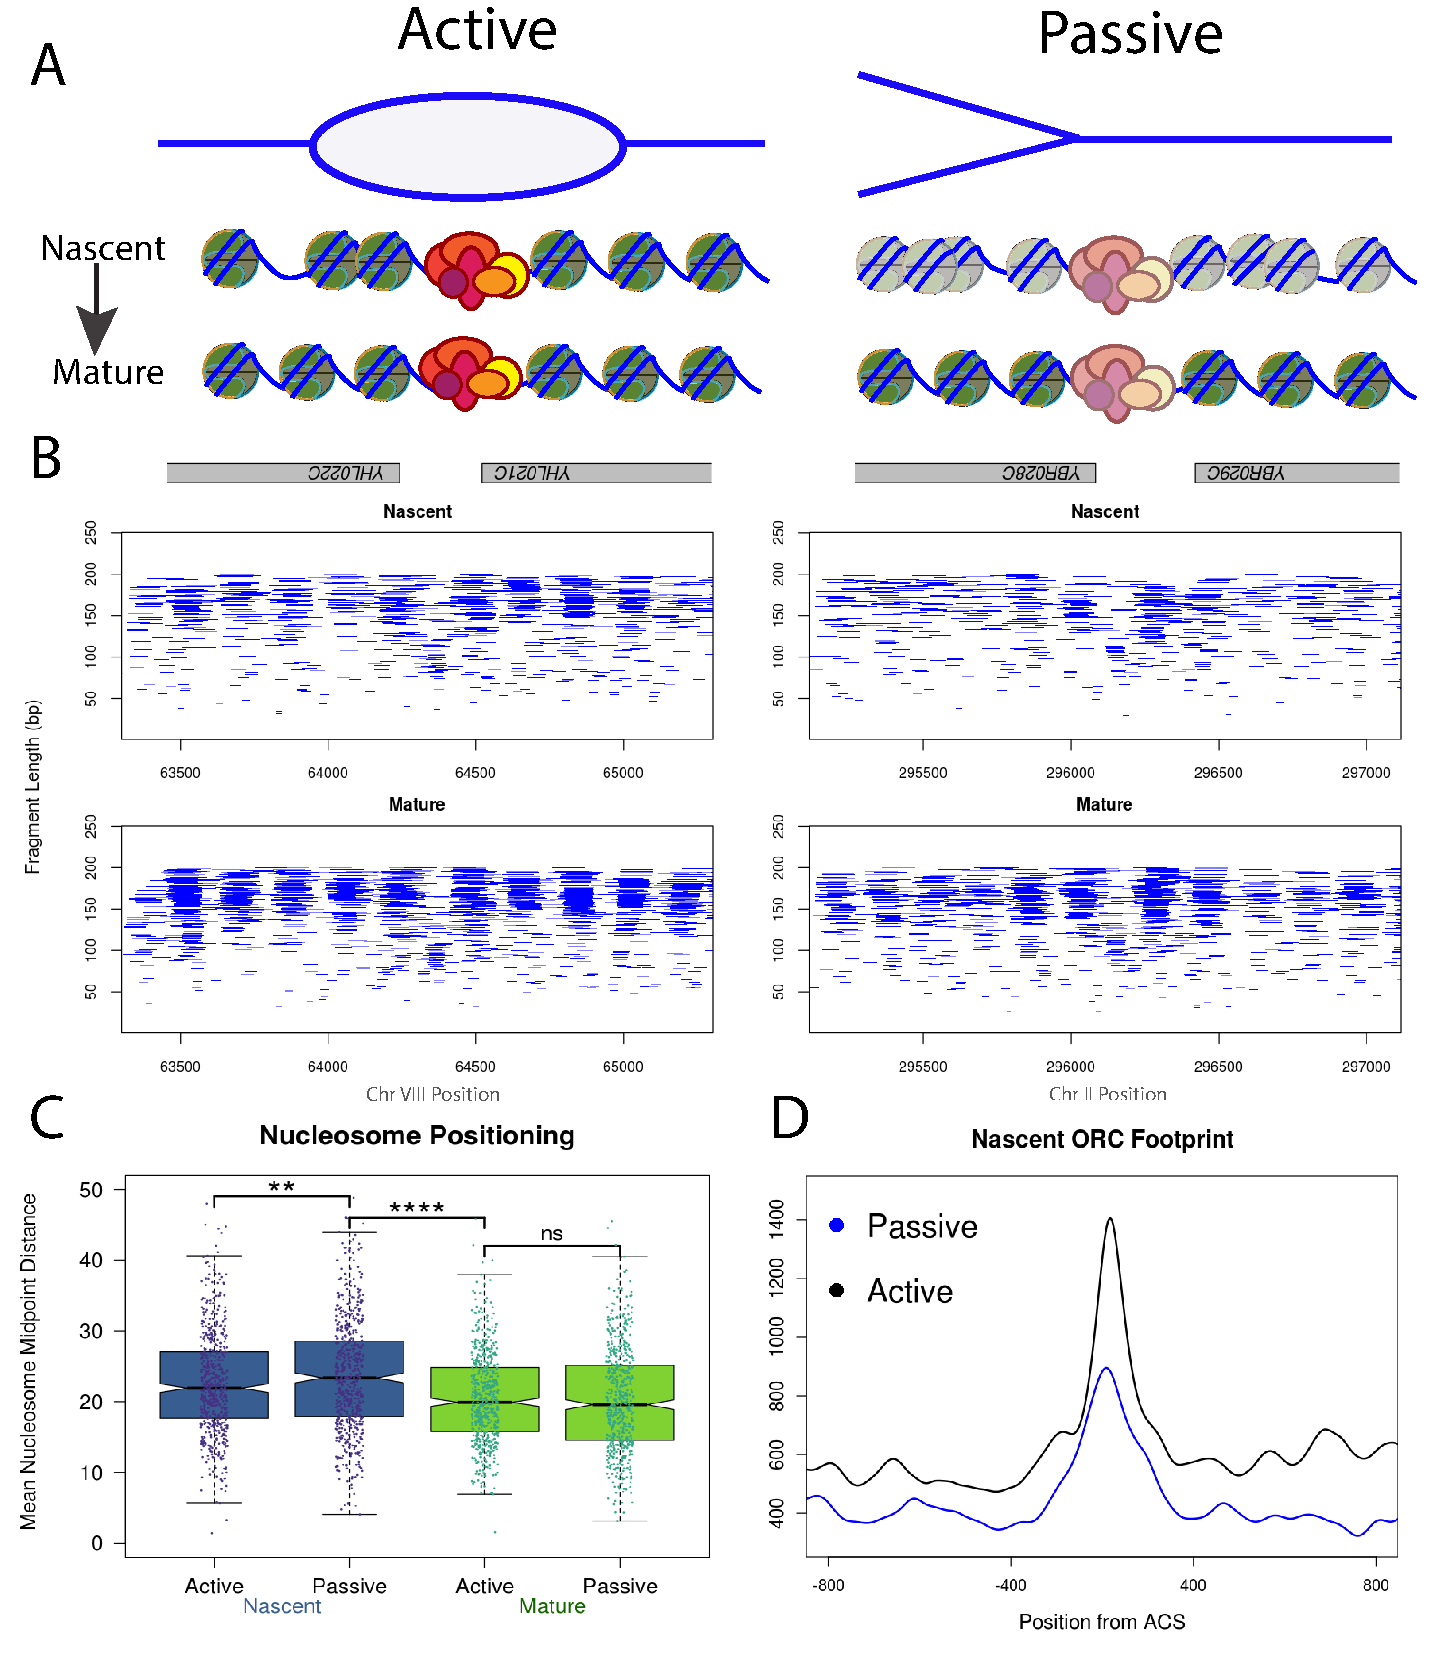
\includegraphics[width=3.5in]{r35_figures/dave_origin_cartoon_COMPLETE_figure_10_1_17_2.pdf}
\end{center}
\vspace{3mm}
\caption{Chromatin assembly at actively and passively replicated origins.  A. Model depicting nascent and mature chromatin organization at active or passive  origins.  B. GCOPs of nascent and mature chromatin at \texit{ARS805} (active) and \textit{ARSII-294} (passive).  The nascent chromatin at the passively replicated origin has more disorganized chromatin.  C.  Quantification of nucleosome positioning (median distance of nucleosome midpoints from bulk chromatin) for active and nascent chromatin at active (n=100) and passive origins (n=100).  D.  ORC footprint occupancy in nascent chromatin at active and passive origins.}%
\end{floatingfigure}%

\ssheading{Re-establishment of chromatin architecture at actively and passively replicating origins}  
A consequence of the temporal order of the DNA replication program is that some origins actively initiate DNA replication whereas other origins are passively replicated by the traveling replication fork.  We sought to identify and compare the kinetics of chromatin maturation at active and passive replication origins.  We hypothesized that the chromatin dis-assembly and assembly mechanisms at the elongating fork may be different from a local initiation event.  By coupling our genome-wide chromatin occupancy profiles (GCOPs) with EdU pulse-labeling of nascent and mature chromatin, we were able to interrogate nascent and mature chromatin structure at actively and passively replicated origins.  We found that the nascent chromatin structure surrounding active replication origins was significantly more organized than nascent chromatin at passive origins ({\color{dukeblue}\textbf{Figure 1}}).  However, the mature chromatin at both active and passive origins had returned to its default state of well-positioned nucleosomes surrounding the origin.  These results suggest that there are inherent differences in chromatin re-assembly at  active origins versus those that are passively replicated.  One hypothesis that we will explore is that following initiation there is a mechanism to retain ORC at active origins whereas at passive origins, ORC is displaced by the replication fork and then remains in competition with nucleosomes to re-establish origin specific chromatin architecture.  The rapid re-establishment of chromatin architecture surrounding active origins may provide a positive feed back loop to promote early and efficient origin activation. 
\begin{floatingfigure}[r]{3.4in}
\vspace{-15mm}
\begin{center}
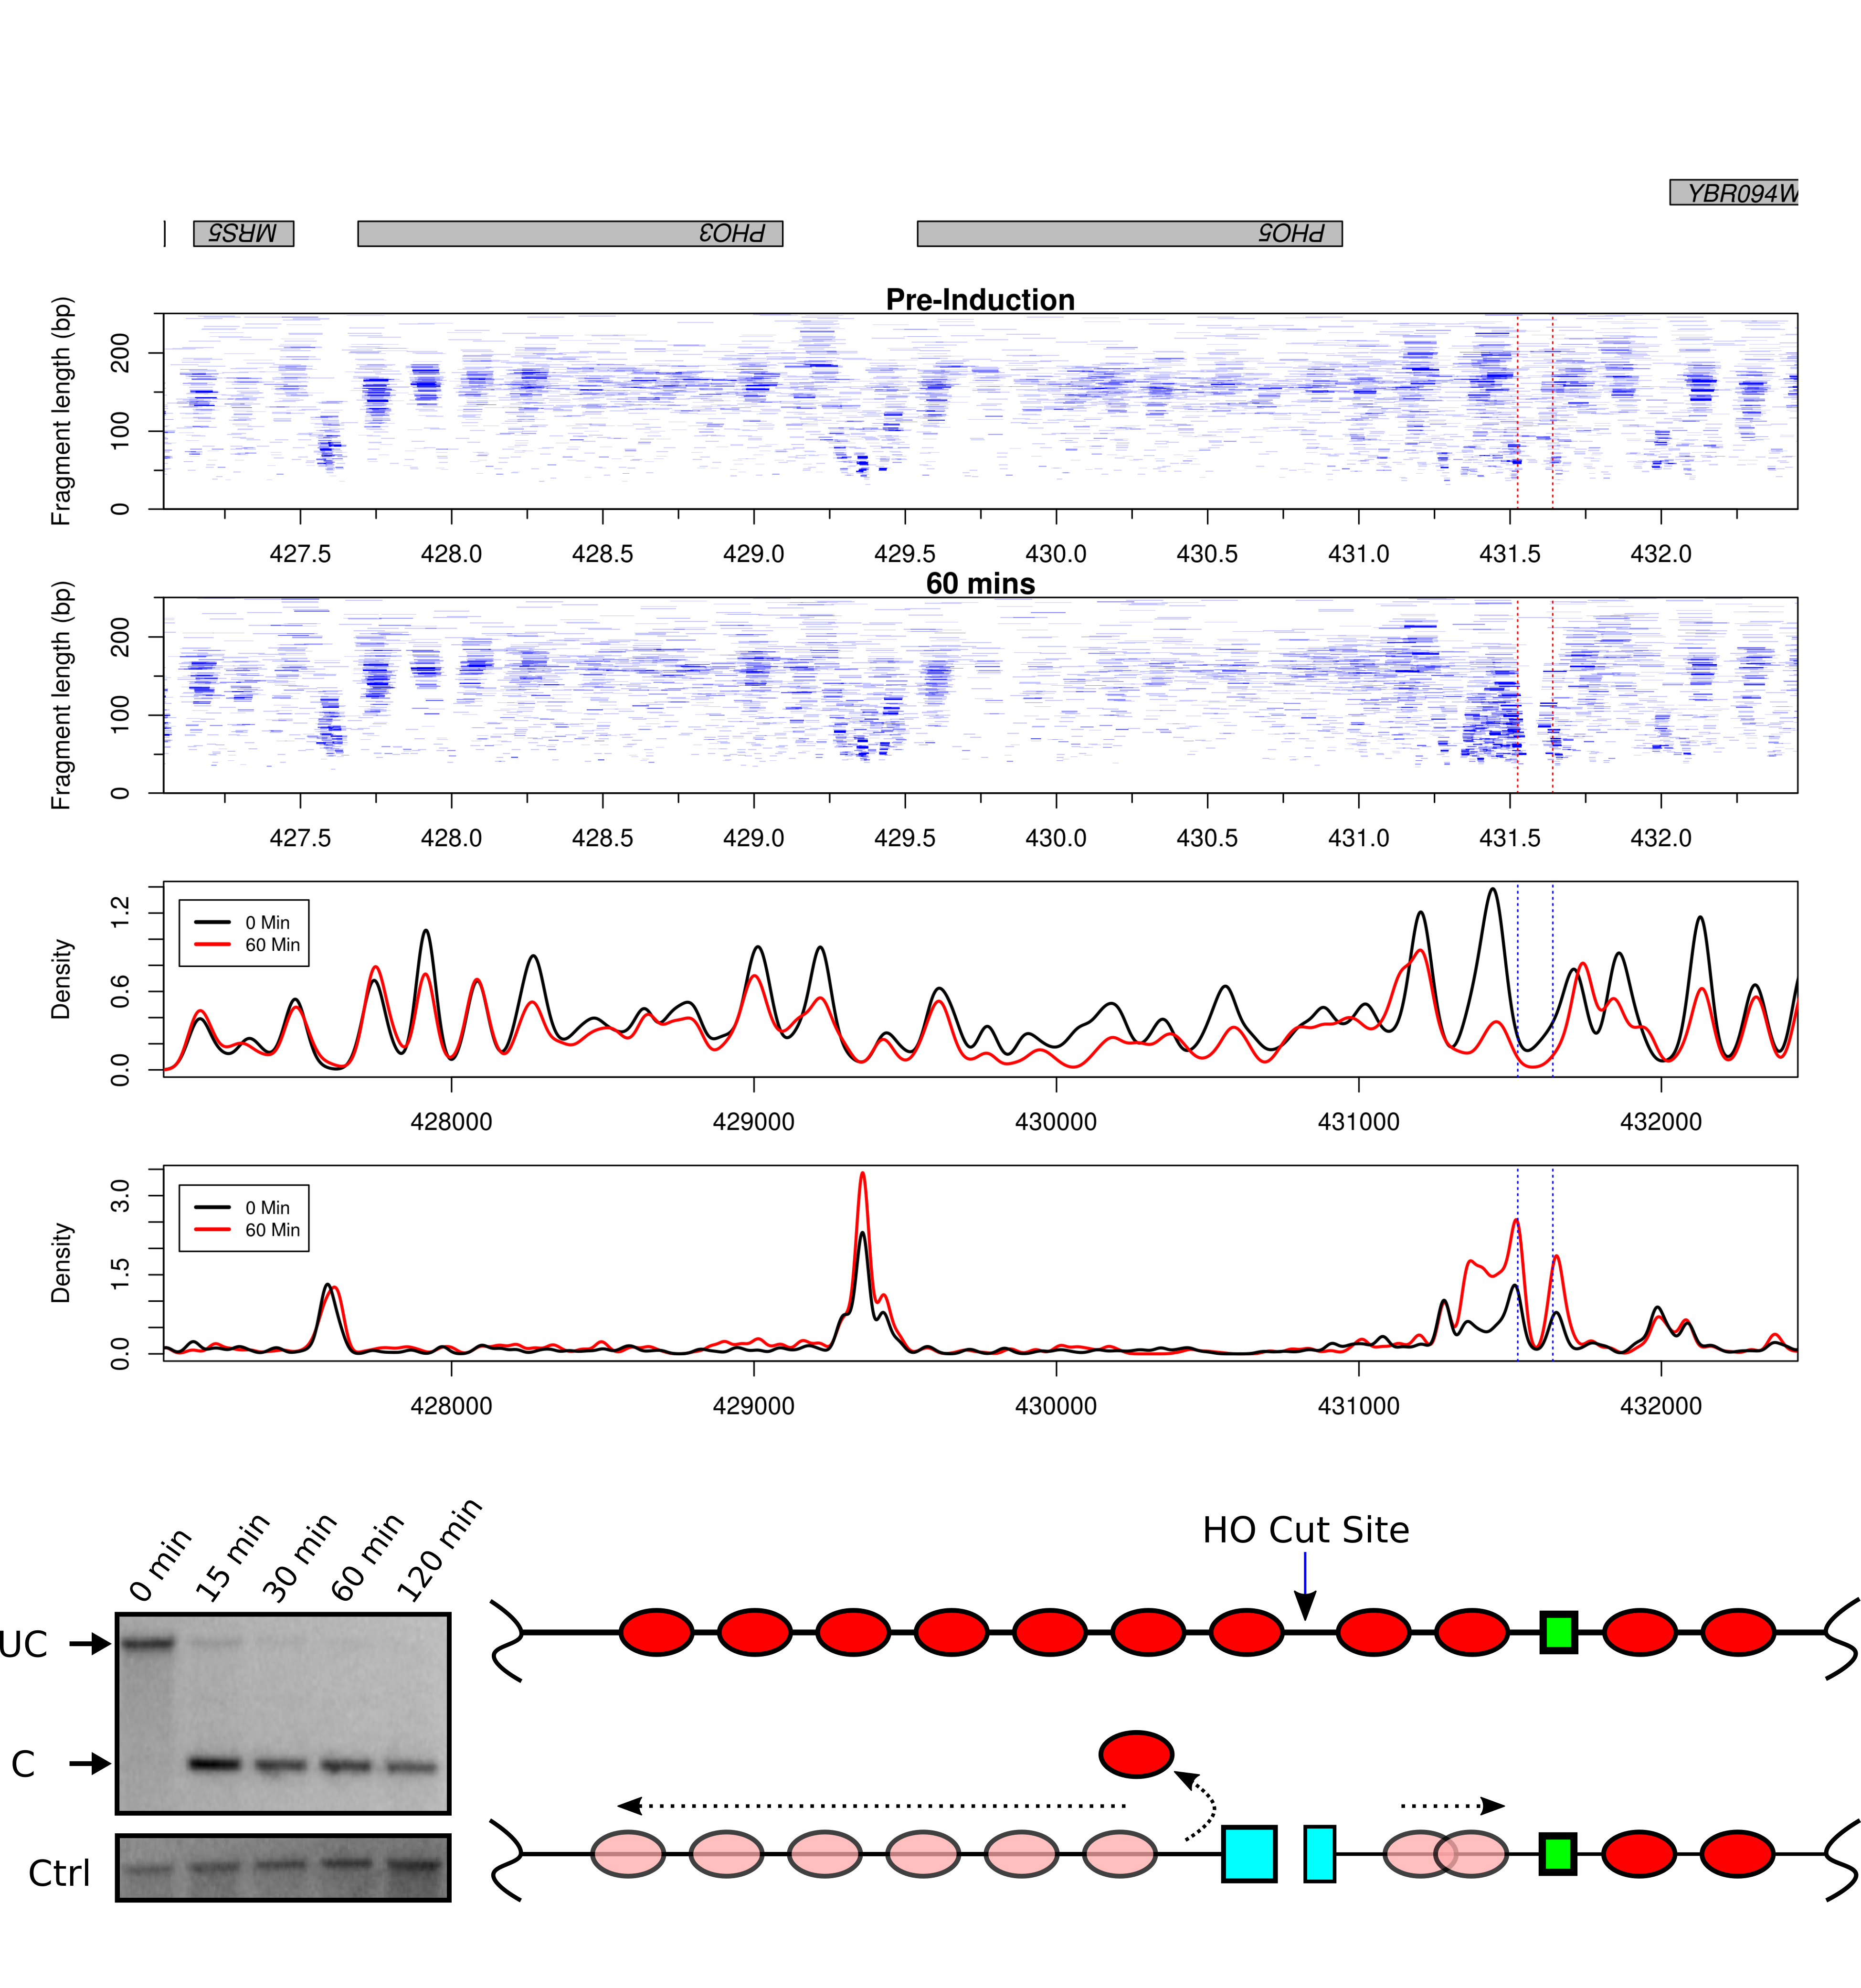
\includegraphics[width=3.4in]{r35_figures/vinay_pho5.png}
\end{center}
\vspace{3mm}
\caption{Pho5 in hte house}%
\end{floatingfigure}%

\ssheading{Chromatin architecture at DNA breaks}
 We have integrated ectopic HO endonuclease recognition sites at multiple loci throughout the genome in order to assess how the local chromatin is impacted following the induction and subsequent repair of site-specific breaks.  Perhaps not surprising, we have found a large variance in the kinetics by which different ectopic HO endonuclease recognition sites are cleaved by Gal-HO.  For example, upstream of \textit{PHO5} we observe $>$90\% cutting within 15 minutes, whereas at the \textit{ERV46} locus, cleavage is significantly reduced to $\sim$20\% during the same time interval.  These data are consistent with the local chromatin organization limiting the accessibility of the endonuclease recognition site.  We will use our GCOP assay to profile the chromatin surrounding the ectopic insertions to better understand how chromatin architecture facilitates recognition and cleavage by the HO endonuclease. The insights gained from our ability to profile chromatin accessibility at nucleotide resolution may be informative for improving the efficacy of gene editing approaches in higher eukaryotes.

In order to follow the replication independent changes in chromatin structure immediately following a break and its subsequent repair by NHEJ, it is important that we can rapidly induce a double strand break by Gal-HO and quickly repress Gal-HO to assess repair kinetics.  We are able to hold haploid cells in a G1 $\alpha$-factor mediated arrest, induce cutting for 30 minutes at \textit{PHO5} ($>$95\% cutting efficiency), turn off Gal-HO and observe that more than 70\% of the cleavage products are restored by 4 hours in the absence of a donor template.  We will explicitly confirm that the repair we observe is due to NHEJ and thus \textit{DNL4}-dependent.  These experiments will not only provide a detailed temporal view of chromatin changes associated with DNA damage and repair, but will also provide a platform to explicitly test the local and direct role of key repair factors and chromatin remodeling enzymes in the process.